\documentclass[border=10pt]{standalone}
\usepackage{tikz}
\usetikzlibrary{arrows.meta, positioning, fit, backgrounds}
\usepackage{xcolor}

% Brand colors
\definecolor{Garnet}{HTML}{73000A}
\definecolor{Atlantic}{HTML}{466A9F}
\definecolor{Congaree}{HTML}{1F414D}
\definecolor{Horseshoe}{HTML}{65780B}
\definecolor{Rose}{HTML}{CC2E40}
\definecolor{Honeycomb}{HTML}{A49137}
\definecolor{LightGray}{HTML}{ECECEC}
\definecolor{Black90}{HTML}{363636}

\begin{document}
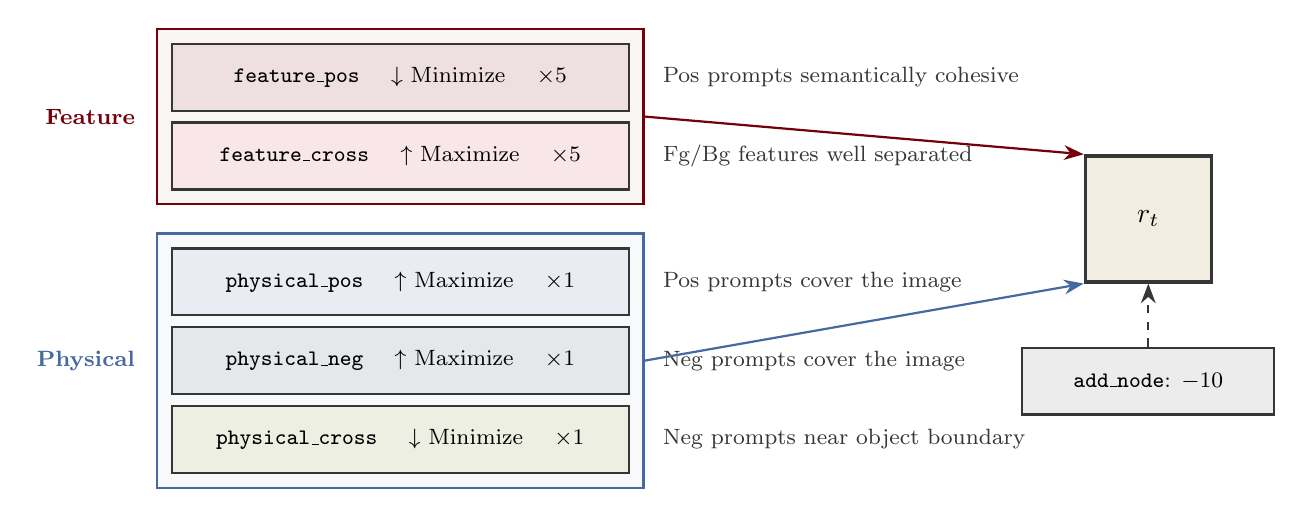
\begin{tikzpicture}[
    comp/.style={
        draw=Black90, thick, minimum width=5.8cm, minimum height=0.85cm,
        align=center, font=\footnotesize, inner xsep=6pt
    },
    desc/.style={
        font=\footnotesize, anchor=west, text=Black90
    },
    arr/.style={-{Stealth[length=2.5mm]}, thick},
    every node/.style={font=\footnotesize}
]

% === Feature Space components ===
\node[comp, fill=Garnet!12] (r1) at (0, 2.4)
    {\texttt{feature\_pos} \quad $\downarrow$ Minimize \quad $\times 5$};
\node[comp, fill=Rose!12] (r2) at (0, 1.4)
    {\texttt{feature\_cross} \quad $\uparrow$ Maximize \quad $\times 5$};

% === Physical Space components ===
\node[comp, fill=Atlantic!12] (r3) at (0, -0.2)
    {\texttt{physical\_pos} \quad $\uparrow$ Maximize \quad $\times 1$};
\node[comp, fill=Congaree!12] (r4) at (0, -1.2)
    {\texttt{physical\_neg} \quad $\uparrow$ Maximize \quad $\times 1$};
\node[comp, fill=Horseshoe!12] (r5) at (0, -2.2)
    {\texttt{physical\_cross} \quad $\downarrow$ Minimize \quad $\times 1$};

% === Descriptions (right of each row) ===
\node[desc, right=0.3cm of r1] {Pos prompts semantically cohesive};
\node[desc, right=0.3cm of r2] {Fg/Bg features well separated};
\node[desc, right=0.3cm of r3] {Pos prompts cover the image};
\node[desc, right=0.3cm of r4] {Neg prompts cover the image};
\node[desc, right=0.3cm of r5] {Neg prompts near object boundary};

% === Group labels ===
\begin{scope}[on background layer]
\node[draw=Garnet, thick, fill=Garnet!4, inner sep=5pt, fit=(r1)(r2)] (gf) {};
\node[draw=Atlantic, thick, fill=Atlantic!4, inner sep=5pt, fit=(r3)(r4)(r5)] (gp) {};
\end{scope}

\node[font=\footnotesize\bfseries, text=Garnet, anchor=east] at ([xshift=-4pt]gf.west) {Feature};
\node[font=\footnotesize\bfseries, text=Atlantic, anchor=east] at ([xshift=-4pt]gp.west) {Physical};

% === Sum node (centered between the two groups) ===
\node[draw=Black90, very thick, fill=Honeycomb!15,
      minimum width=1.6cm, minimum height=1.6cm,
      align=center, font=\normalsize] (sum) at (9.5, 0.6) {$r_t$};

% === Arrows from groups to sum ===
\draw[arr, Garnet] (gf.east) -- (sum.north west);
\draw[arr, Atlantic] (gp.east) -- (sum.south west);

% === Penalty ===
\node[comp, fill=LightGray, minimum width=3.2cm, below=0.8cm of sum] (pen)
    {\texttt{add\_node}: $-10$};
\draw[arr, dashed, Black90] (pen.north) -- (sum.south);

\end{tikzpicture}
\end{document}
